\chapter{Grundlagen}
Dieses Kapitel verschafft einen Überblick über die benötigten theoretische Grundlagen, um die Methoden dieser Arbeit zu verstehen. 
Als erstes wird eine Einführung in Neuronale Netzwerke gegeben, anschließend werden
einzelne Bestandsteile und Varianten von Neuronalen Netzwerken erklärt. 
Als nächstes wird der ``Lab-Farbraum'' kurz erklärt. Abschließend wird einen Überblick über verwandte Arbeiten gegeben.

\section{Neuronale Netze}
Künstliche Neuronale Netze sind inspiriert durch das Menschliche Gehirn und werden für Künstliche Intelligenz und Maschinelles Lernen
angewendet. Sie werden für überwachtes und unüberwachtes lernen verwendet. In der vorliegende Arbeit werden nur Methoden des überwachtes 
lernen angewendet. Bei überwachtes lernen sind die Datensätze gelabelt sodass den Output von dem Neuronales Netz mit den richtigen Ergebnissen
verglichen werden kann.
\\
\\
Neuronale Netze bestehen aus Neuronen oder auch ``Units'' genannt, die Schichtenweise in ``Layers'' (Schichten) angeordnet sind.
Beginnend mit der Eingabeschicht (Input \gls{Layer}) fließen Informationen über eine oder mehrere Zwischenschichten (Hidden \gls{Layer}) bis hin zur 
Ausgabeschicht (Output \gls{Layer}). Dabei ist der Output des einen Neurons der Input des nächsten. \cite{neuronale-netze-aufbau}

\subsection{Feedforward Neural Network}
Das Ziel von einem Feedforward Neural Network ist die Annäherung an irgendeine Funktion $ f^* $. Ein Feedforward Neural Network definiert 
eine Abbildung $ y = f(x;W) $ wobei $ x $ den Input ist und $ W $ die lernbare Parameter sind (auch Gewichte genannt).
\cite[164-223]{Goodfellow-et-al-2016}
\\
\\
Diese Netzwerkarchitektur heißt ``feedforward'' weil der Informationsfluss von der Input \gls{Layer} über die Hidden Layers bis zur Output \gls{Layer} 
in einer Richtung weitergereicht wird.

Feedforward Neural Networks werden als eine Kette von Funktionen repräsentiert. Als Beispiel,
kann man die Funktionen $ f^{(1)}, f^{(2)}, f^{(3)} $ in Form einer Kette verbinden um $ f(\textbf{x}) = f^{(3)}(f^{(2)}(f^{(1)}(\textbf{x}))) $
zu bekommen. Diese Kettenstrukturen sind die am häufigsten genutzte Struktur bei Neuronale Netzwerke. In diesem Fall, $ f^{(1)} $ ist das 
erste Layer, $ f^{(2)} $ das zweite und $ f^{(3)} $ der Output Layer von diesem Netzwerk. Die Länge dieser Kette definiert die Tiefe von
einem Netzwerk. Je tiefer
ein Netzwerk ist desto mehr lernbare Parameter hat es und somit eine erhöhte Rechenleistung braucht um trainiert zu werden.
In der Praxis werden die Netzwerke sehr tief, daher der Begriff Deep Learning.
\\
\\
Während dem Training werden die Gewichte von $ f(x) $ verstellt, um $ f^*(x) $ zu erhalten. Jedes Trainingsbeispiel $ x $ ist mit einem Label
$ y = f^*(x)$ versehen. Die Trainingsbeispiele legen genau fest, was der Output Layer generieren soll. Der Output Layer soll Werte generieren,
die nah an $ y $ liegen. Das Verhalten von den Hidden Layers wird nicht durch die Trainingsbeispiele festgelegt, sondern der Lernalgorithmus
soll definieren, wie diese Layers verwendet werden, um die beste Annäherung von $ f^*(x) $ zu generieren.

\subsection{Fully-connected Neural Network}
Fully-connected Neural Networks sind die am häufigsten vorkommende Art von Neuronale Netze. In dieser Netzwerkarchitektur sind alle Neuronen
von einem Layer mit alle Neuronen von der vorherige und nächsten Layer verbunden. Neuronen in dem gleichen Layer sind aber nicht miteinander verbunden.
\cite{cs231-neural-networks}

\begin{figure}[H]
  \centering
  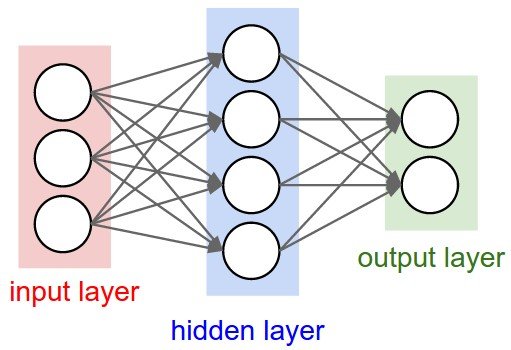
\includegraphics[width=0.65\textwidth]{resources/nn/neural_net.jpeg}
  \caption{
    Fully-connected Neural Network mit 2 Layers (ein Hidden Layer mit 4 Neuronen) und ein Output Layer mit 2 Neuronen 
    \cite{fully-connected-neural-network}
  }
  \label{image:neuronal-network}
\end{figure}

% TODO: Formel erklären, Formel und Elemente der Formel erklären

Eine der wichtigsten Gründe für die Anordnung von Neuronale Netze in Layers ist dass so eine Struktur anhand von Matrix Multiplikationen
berechnet werden kann. Das obere Bild \ref{image:neuronal-network} stellt ein Netzwerk mit 3 Inputs $ x $, eine Hidden Layer mit 4 Neuronen
und eine Output Layer mit 2
Neuronen dar. Die Kreisen repräsentieren die Neuronen und einem Bias Wert $ b $, die Pfeilen stellen die Gewichte $ w $ dar.

\begin{align}
  f(x) = w*x + b
\end{align}

Nach jeden Hidden Layer läuft den Output durch eine Aktivierungsfunktion $ \sigma $ die in \ref{subsection:aktivierungsfunktionen} erklärt wird.
Daraus wird die vorherige Formel um $ \sigma $ erweitert:

\begin{align}
  f(x) = \sigma( w*x + b)
\end{align}

\subsubsection{Forward Pass}
Den Forward Pass von einem Neuronalem Netz wird anhand von Matrizen Multiplikationen berechnet. Um das zu veranschaulichen wird
es anhand eines Beispiels erklärt.

Ausgehend von einem Netzwerk mit 3 Inputs, eine Hidden Layer mit 2 Neuronen und einem Output Neuron, ergeben sich folgende Beispielwerte:
\begin{equation} 
  \vspace{5pt}
  X = \begin{pmatrix}
    1 &0 &1 &1 \\
    1 &1 &1 &0 \\
    1 &1 &0 &1
  \end{pmatrix} 
  \hspace{5pt}
  W = \begin{pmatrix}
    10 &20 \\
    -20 &-40 \\
    20 &0 \\
    -40 &0
  \end{pmatrix}
  \hspace{5pt}
  W_{out} = \begin{pmatrix}
    20 \\
    40 \\
    -40
  \end{pmatrix}
\end{equation}

$ X $ sind die Inputs, $ W $ die Gewichte von dem Hidden Layer und $ W_{out} $ die Gewichte von dem Output Layer.
Die erste Spalte in dem Input $ X $ und die erste Zeile in beide Gewichtsmatrizen $ W $ und $ W_{out} $ sind die Werte für den Bias.
Diese Anordnung von den Bias Werte ermöglicht die Berechnung durch eine einzigen Matrix Multiplikation. Als Aktivierungsfunktion wird ReLU 
\cite{10.5555/3104322.3104425} verwendet:

\begin{equation}
  \vspace{5pt}
  f(x) = 
  \begin{cases}
    0 &\text{if \(x < 0\)}  \\
    x &\text{if \(x \geq 0\)} 
  \end{cases}
\end{equation}

Im ersten Schritt durchläuft den Input durch das Hidden Layer $ f(X \times W) $:
\begin{equation}
  \vspace{5pt}
  f \left(
  \begin{pmatrix}
    1 &0 &1 &1 \\
    1 &1 &1 &0 \\
    1 &1 &0 &1
  \end{pmatrix}
  \times
  \begin{pmatrix}
    10 &20 \\
    -20 &-40 \\
    20 &0 \\
    -40 &0
  \end{pmatrix}
  \right)
  =
  \begin{pmatrix}
    0 &1 \\
    1 &0 \\
    0 &0
  \end{pmatrix}
\end{equation}

Im zweiten Schritt wird den Output von der vorherige Multiplikation mal die Gewichte von dem Output Layer multipliziert:
\begin{equation}
  \vspace{5pt}
  f \left(
  \begin{pmatrix}
    1 &0 &1 \\
    1 &1 &0 \\
    1 &0 &0
  \end{pmatrix}
  \times
  \begin{pmatrix}
    20 \\
    40 \\
    -40
  \end{pmatrix}
  \right)
  =
  \begin{pmatrix}
    0 \\
    1 \\
    0
  \end{pmatrix}
\end{equation}

\subsection{Aktivierungsfunktionen}\label{subsection:aktivierungsfunktionen}
Eine Aktivierungsfunktion definiert die Aktivierungsrate von einem Neuron. Es gibt verschiedene Aktivierungsfunktionen:

% TODO: Formeln mit nummerierung
\subsubsection{Sigmoid}
Sigmoid ist eine nicht lineare Funktion welche die Werte in einem Wertebereich von $ [0, 1] $ bringt.
Große negative Werte werden annähernd 0 und große positive Werte werden annähernd 1. Sigmoid hat verschiedene Nachteile, es neigt dazu den Gradienten zu verschwinden
und die Outputs sind nicht Null zentriert. Sigmoid ist definiert als:

\begin{equation}
  \sigma(x) = \frac{1}{1 + e^{-x}}
\end{equation}

wobei $x$ einem Input ist.

\begin{figure}[H]
  \centering
  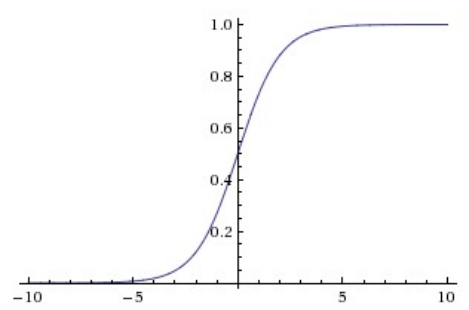
\includegraphics[width=0.65\textwidth]{resources/nn/sigmoid.png}
  \caption{
    Sigmoid Aktivierungsfunktion 
    \cite{neuron-model}
  }
  \label{image:sigmoid}
\end{figure}

% \subsubsection{Tanh}
% Die Tanh Aktivierungsfunktion bringt Werte in einem Wertebereich von $ [-1, 1] $. Es ist eine skalierte Sigmoid ($ \sigma $) Funktion,
% $ tanh(x) = 2\sigma(2x) - 1 $. Die Nachteile von Tanh sind ähnlich zu Sigmoid aber der Output ist Null zentriert.

% \begin{figure}[H]
%   \centering
%   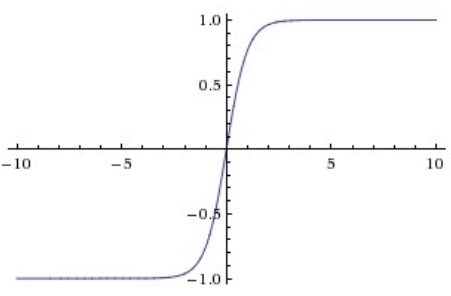
\includegraphics[width=0.65\textwidth]{resources/nn/tanh.png}
%   \caption{
%     Tanh Aktivierungsfunktion 
%     \cite{neuron-model}
%   }
%   \label{image:tanh}
% \end{figure}

\subsubsection{ReLU}
Die Rectified Linear Unit konvertiert alle negative Werte in 0 und alle positive Werte behalten deren Identität. Diese Aktivierungsfunktion
wurde für die Netzwerke in dieser Arbeit benutzt da es Vorteile gegenüber Sigmoid zeigt. Einer der Vorteile ist dass die Mathematische
Auswertung der Funktion unkompliziert ist. Außerdem beschleunigt es die Konvergenz von Stochastisches Gradientenabstiegsverfahren im Vergleich zu Sigmoid.
ReLU ist definiert als:

\begin{equation}
  f(x) = max(0, x)
\end{equation}

wobei $x$ einem Input ist.
\\
Neuronen die ReLU als Aktivierungsfunktion verwenden, können während des Trainings ``sterben''. Zum Beispiel, wenn der Gradient in einem Neuron
zu groß ist, kann dieser zu einem update der Gewichte führen, wo das Neuron nie wieder aktiviert werden kann. Mit einer korrekter Einstellung der
Lernrate kann das vermieden werden. \cite{cs231-neural-networks}

\begin{figure}[H]
  \centering
  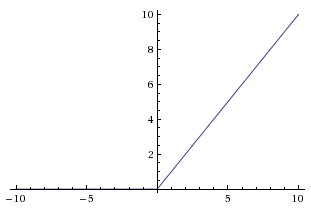
\includegraphics[width=0.65\textwidth]{resources/nn/relu.jpeg}
  \caption{
    Rectified Linear Unit (ReLU) 
    \cite{neuron-model}
  }
  \label{image:relu}
\end{figure}

% TODO: alpha durch was anderes ersetzen
% \subsubsection{Leaky ReLU}
% Leaky ReLU ist einer Variante von ReLU, die versucht, das Problem mit den ``sterbenden'' Neuronen zu minimieren. Anstatt alle negative Werte
% in Null zu konvertieren, werden die Werte mal einer Konstante multipliziert. Die Funktion wird zu $ f(x) = 1(x < 0)(\alpha x) + 1(x >= 0)(x)$,
% wobei $ \alpha $ eine Konstante mit geringeren Wert ist, zum Beispiel $ 0.001 $.

% \begin{figure}[H]
%   \centering
%   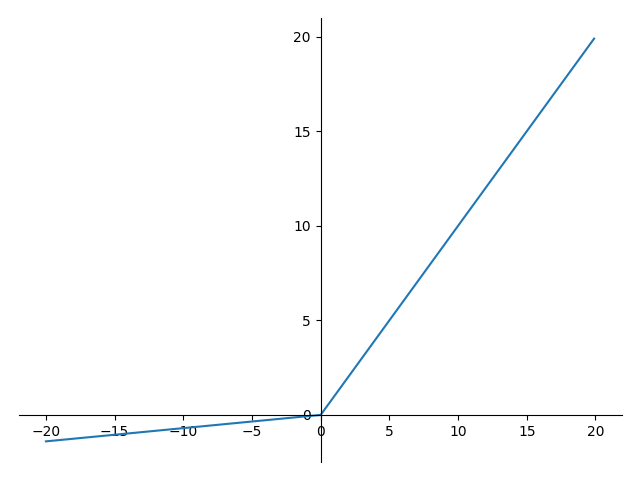
\includegraphics[width=0.65\textwidth]{resources/nn/leaky-relu.png}
%   \caption{
%     Leaky ReLU 
%     \cite{leaky-relu}
%   }
%   \label{image:leaky-relu}
% \end{figure}

\subsection{Convolutional Neural Networks}
Convolutional Neural Networks (\gls{CNN}) sind eine besondere Form von künstliche neuronale Netzwerke, das speziell für 
die Verarbeitung von Bilddaten, unter anderen, vorgesehen ist \cite{convnet-erklaerung}.
\\
Im gegensatz zu traditionelle neuronale Netzwerke, die ein Vektor als Input nehmen, nehmen Convolutional Neural Networks ein 3D Volumen als Input
($ W \times H \times C $, wobei $W$ die Breite, $H$ die Höhe und $C$ die Farbkanäle sind).

\begin{figure}[H]
  \centering
  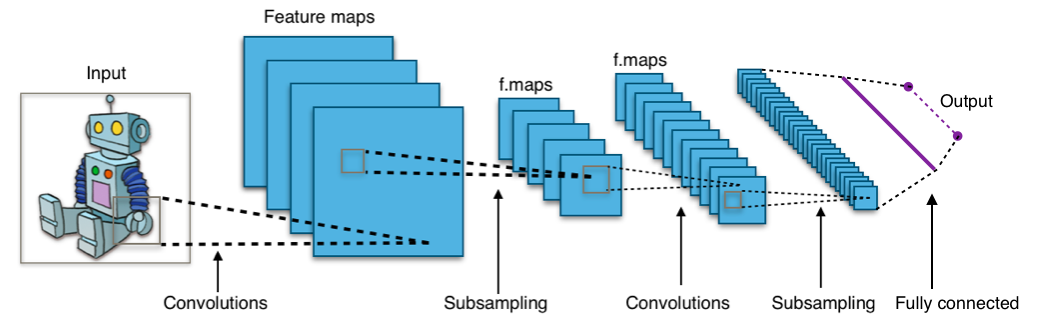
\includegraphics[width=1\textwidth]{resources/cnn/typical_cnn.png}
  \caption{
    Typische Struktur von einem Convolutional Neural Network
    \cite{typical_cnn_img}
  }
  \label{image:typical_cnn_img}
\end{figure}


\gls{CNN}s bestehen in der Regel aus 2 Formen von \gls{Layer}s, die Convolutional \gls{Layer} und die Pooling Layer. 
\\
\\
Die Convolutional \gls{Layer} besteht aus mehrere hintereinander geschaltete 3 Dimensionale
Filter, auch Kernel genannt ($ W \times H \times D$, wobei $D$ die Tiefe der Feature maps darstellt), die während den Forward pass, über dem Bild 
mit einer festgelegten Schrittweite (\gls{stride}), geschoben werden. Mit den sogenannten Padding wird der Verhalten an den Rändern festgelegt.
An jeder stelle wird eine Matrix Multiplikation zwischen den Filter und die aktuelle Position auf dem Bild durchgeführt. 
Als Output wird eine 2 Dimensionalen Feature maps generiert. Die Größe dieser Feature map ist abhängig 
von der Größe des Filters, dem Padding und vor allem dem \gls{stride}. Ein \gls{stride} von 2 bei einer Filter Größe von $ 2\times2 $ führt beispielsweise 
pro Filter zu einer Halbierung der Größe der Feature map im Vergleich zum Input Volumen \cite{aufbau-funktion-convnet}.
Ein \gls{stride} von 1 bei einem $ 3\times3 $ Filter mit Padding 1 führt zu einer Feature map mit der gleiche Größe wie der Input Volumen.
\\
\\
Die Filter erkennen in den ersten Ebenen einfache Strukturen wie Linien, Farben oder Kanten. In den nächsten Ebenen lernt das CNN Kombinationen aus 
diesen Strukturen wie Formen oder Kurven. In den tieferen \gls{Layer}s werden komplexere Strukturen und Objekte identifiziert. 

\begin{figure}[H]
  \centering
  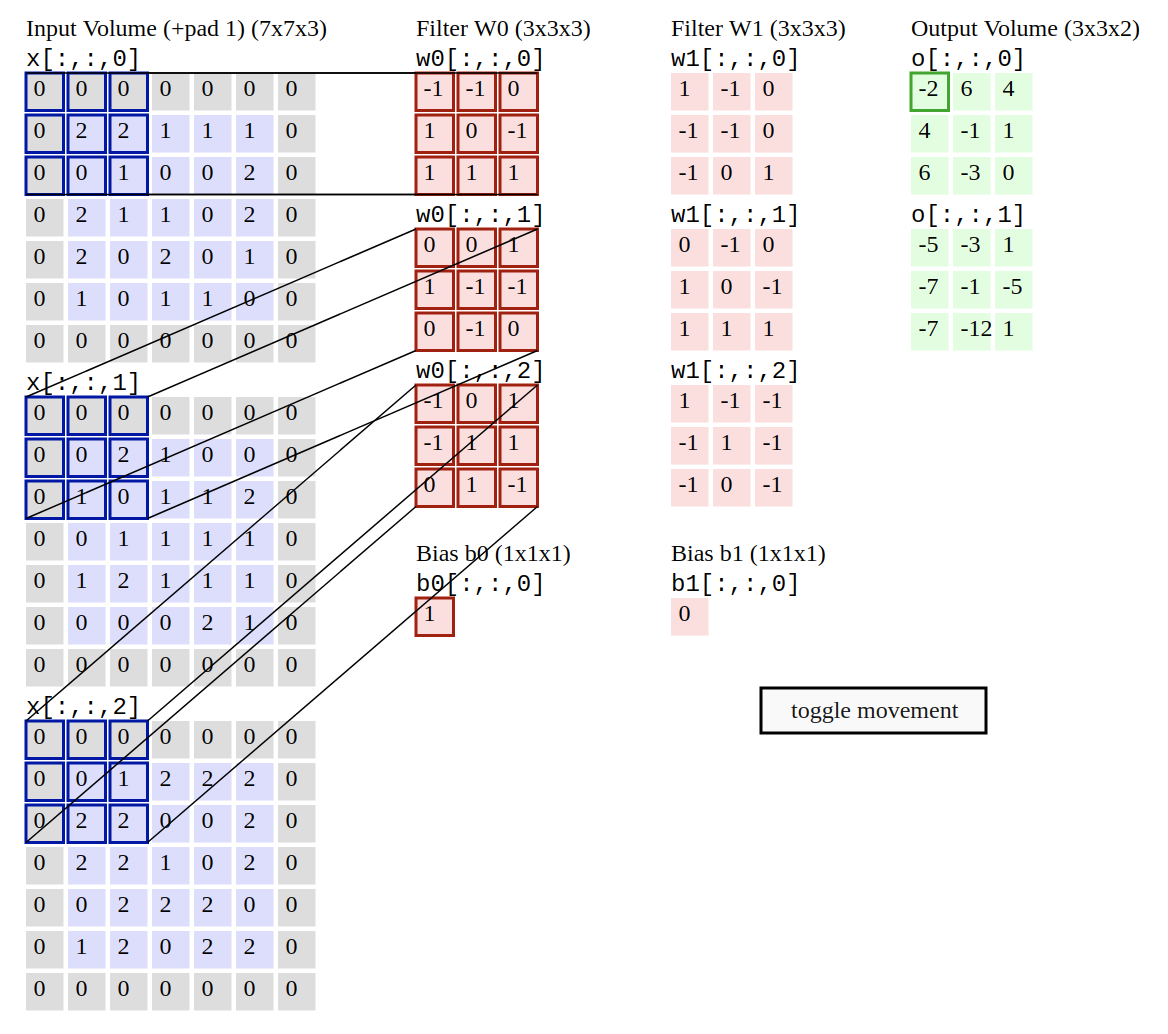
\includegraphics[width=0.75\textwidth]{resources/cnn/funktion-cnn.png}
  \caption{
    Beispiel Forward pass von einem Convolutional \gls{Layer} mit einem $ 7\times7\times3 $ Input Volumen, zwei $3\times3\times3$ Filter, 
    Padding 1 und \gls{stride} 2.
    \cite{convnet-demo}
  }
  \label{image:convnet-demo}
\end{figure}

Die Pooling Layer dient zur Reduktion der Dimensionen von einem Input Volumen und somit die Parameter von dem Netzwerk. Es gibt 
verschiedene Pooling Operationen die angewendet werden können, wie zum Beispiel Maximum Pooling, Minimum Pooling, oder Average Pooling. Im Rahmen 
dieser Arbeit wird Maximum Pooling (oder Max Pooling) verwendet.
\\
\\
Ein Max Pooling \gls{Layer} aggregiert die Aktivierungsmatrizen von Convolutional Layers, in dem nur die höchste Zahl von einem Filter weitergegeben 
wird. Zum Beispiel, bei einem $ 2 \times 2 $ Filter wird aus 4 Zahlen nur 1 Zahl weitergegeben. Damit wird einer Reduktion der Dimensionen erreicht.

\begin{figure}[H]
  \centering
  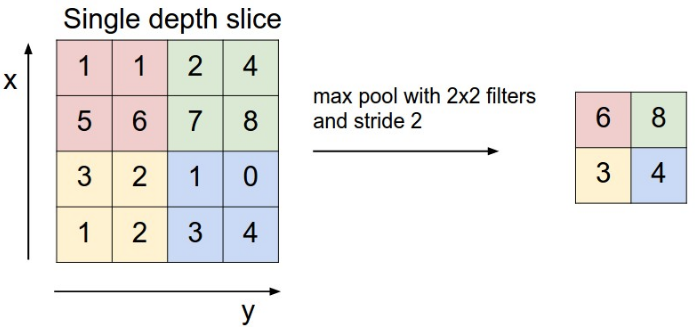
\includegraphics[width=0.75\textwidth]{resources/cnn/pooling.png}
  \caption{
    Max pooling Operation mit $ 2 \times 2 $ Filtern und \gls{stride} 2
    \cite{convnet-demo}
  }
  \label{image:pooling}
\end{figure}

\subsection{Loss Functions}
% Erklärung
Die \gls{loss function} (Kostenfunktion) dient zur Feststellung der Fehler (Loss) zwischen dem Output von einem Model und die Zielwerte. 
Das Ziel von Neuronalen Netzen ist es den Loss zu minimieren. Wenn der Loss gleich Null ist, heißt dass $ y = \hat{y} $. Es gibt verschiedene Arten 
von \gls{loss function}s. Im Rahmen dieser Arbeit werden \gls{loss function}s bezogen auf Regressions– und Klassifizierungsprobleme behandelt.

\subsubsection{Mean Square Error Loss}
Mean Square Error (MSE) Loss misst der mittlere quadratische Fehler und ist definiert als:

\begin{equation}
  J = \frac{1}{N} \sum (y - \hat{y})^2
\end{equation}

wobei, $J$ der Loss ist, $N$ die Anzahl der Klassen, $y$ die Korrekte Klasse (Ground Truth) und $ hat{y}$ die vorhergesagte Klasse ist.

\subsubsection{Cross Entropy Loss}
Der Cross Entropy Loss wird bei Klassifizierungsprobleme verwendet. Es gibt 2 Arten, Binär und Multiclass Cross Entropy Loss. 
Bei der Multiclass Cross Entropy Loss wird ein Vektor mit einer Wahrscheinlichkeitsverteilung $ x \in [0, 1] $ 
ausgewertet, wenn die Korrekte Klasse eine 1 hat ist der Loss 0. Je weniger Wahrscheinlichkeit die Korrekte Klasse besitzt desto höher der Loss 
sein wird. Der Multiclass Cross Entropy Loss ist definiert als: 

\begin{equation}
  J = -\frac{1}{N} \Big(\sum_{i=0}^N y_{i} * \log(\hat{y_{i}})\Big)
\end{equation}

wobei, $J$ der Loss ist, $N$ die Anzahl der Klassen, $y$ die Korrekte Klasse (Ground Truth) und $ \hat{y}$ die vorhergesagte Klasse ist.

\subsubsection{Weighted Cross Entropy Loss}
Bei der Weighted Cross Entropy Loss werden die Klassen gewichtet bevor der Loss berechnet wird. Das ist zum Beispiel nützlich um Klassen  
mit einer niedrige Wahrscheinlichkeit zu bevorzugen.

\subsection{Optimierungsalgorithmen}
Das Ziel von Optimierungsalgorithmen ist eine Kombination von Gewichte $ W $ zu finden, dass die \gls{loss function} minimiert.
Es gibt verschiedene relevante Optimierungsalgorithmen. In der vorliegende Arbeit werden Gradient Descent und Adam verwendet.

\subsubsection{Gradient Descent}
Gradient Descent (Gradientenabstiegsverfahren) ist ein iteratives Verfahren, um bei einer Funktion das Minimum (oder das Maximum) zu finden. 
Mit Hilfe von partielle Ableitungen kann der Gradient von einer Funktion berechnet werden. Ein Gradient ist, in dem Fall von Neuronale 
Netze, ein Vektor der zum höchsten Punkt der \gls{loss function} zeigt. Wird der negative Gradient genommen, zeigt dieser zum tiefsten Punkt.
Bei jeder Kombination von Gewichte wird der Gradient berechnet und mal eine bestimmte Lernrate $ \alpha $ multipliziert, anschließend werden 
alle Gewichte aktualisiert. Die Lernrate definiert die Größe der Schritte in Richtung Minimum. Die Update Regel für die Gewichte ist definiert als:

\begin{equation}
  w_{x+1} = w_x - \alpha * \nabla J(w_x)
\end{equation}

wobei, $w_{x+1}$ die aktualisierte Gewichte sind, $w_x$ die vorherige Gewichte, $ \alpha $ die Lernrate und $\nabla J(w_x)$ der Gradient ist. 
Die Update Regel für den Bias sieht identisch aus.

\begin{figure}[H]
  \centering
  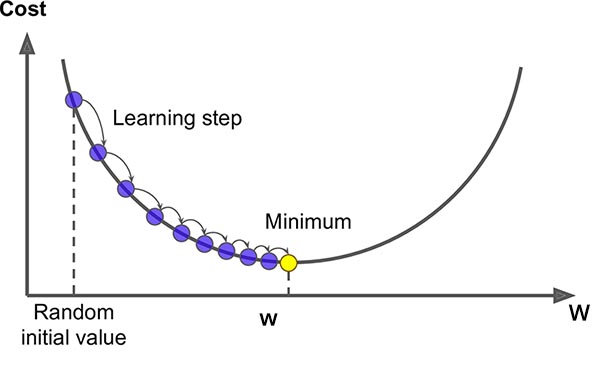
\includegraphics[width=0.65\textwidth]{resources/cnn/gradient-descent.jpg}
  \caption{
    Gradient descent visualisiert
    \cite{gradient-descent}
  }
  \label{image:gradient-descent}
\end{figure}

Es gibt verschiedene Arten von Gradient Descent, Mini-Batch Gradient Descent und Stochastisches Gradient Descent. Bei den normalen Gradient Descent
werden die Gradienten im Bezug zu den gesamten Datensatz berechnet und damit das Update durchgeführt. Mini-Batch Gradient Descent berechnet 
die Gradienten im Bezug zu einen kleinen Teil von dem Datensatz und führt einen Update für alle Parameter durch. Letztendlich, Stochastisches Gradient Descent 
berechnet den Gradient bezogen auf einem einzigen Element von dem Datensatz und führt einen Update für alle Parameter durch.
\\
Um die Konvergenz Richtung Minimum zu beschleunigen, wurde das Gradient Descent mit Momentum entwickelt. Bei diesem Ansatz wird einen 
Geschwindigkeitsparameter zu der Update Regel hinzugefügt die alle vorherige Updates akkumuliert. Das ermöglicht die schnellere Konvergenz mit jedem Schritt.
Die neue Update regel ist definiert als:

\begin{equation}
  \begin{gathered}
    v_{t+1} = \rho v_t - \alpha * \nabla J(w_x) \\
    w_{x+1} = w_x + v_{t+1}
  \end{gathered}
\end{equation}

wobei $v_{t+1}$ der nächste Geschwindigkeitsparameter ist, $v_t$ der aktuelle Geschwindigkeitsparameter und $\rho$ ein Reibungsparameter 
(typisch 0.9) zu Regulierung ist.

% TODO: finish Adam
\subsubsection{Adam}
Adam steht für ``Adaptive Moment Estimation Algorithm'' und ist ein Optimierungsalgorithmus der eine angepasste Lernrate für die verschiedene 
Parameter berechnet \cite{kingma2014adam}. Adam ist der bevorzugte Optimierungsalgorithmus für die vorliegende Arbeit. 
Adam kombiniert die Ansätze von AdaGrad \cite{duchi2011adaptive} und RMSProp. AdaGrad ist eine 
verbesserte Version von Gradient Descent dass eine angepasste Lernrate für die verschiedene Parameter einführt. 



\subsection{Backpropagation}\label{subsection:backpropagation}
Neuronale Netze lernen in dem das Loss minimiert wird. Wie in der vorherigen Sektionen erläutert, bestimmt die \gls{loss function}, 
die Fehlerrate von einem Neuronales Netz. Dieses Loss kann mit Hilfe von einem Optimierungsalgorithmus reduziert werden. 
Backpropagation ermöglicht es, einer effizienten Berechnung der Gradienten in einem neuronalen Netzwerk \cite{was-ist-backpropagation}. 
Mit Hilfe der Kettenregel kann eine Komplexe \gls{loss function} in kleinere Unterfunktionen zerlegt werden um Lokal die Ableitung zu berechnen.
Das ermöglicht eine unkomplizierte Berechnung des Gradienten.
\\
\\
Als Beispiel kann die folgende Sigmoid Funktion in Unterfunktionen zerlegt werden:

\begin{equation}
  f(w,x) = \frac{1}{1+e^{-(w_0 x_0 + w_1 x_1 + w_2)}}
\end{equation}

\begin{figure}[H]
  \centering
  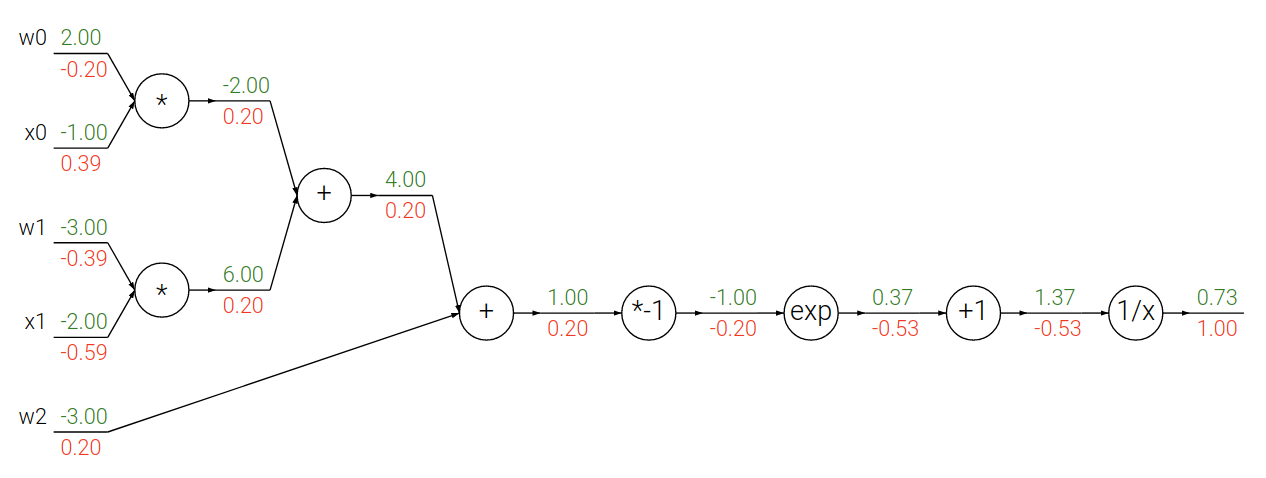
\includegraphics[width=1\textwidth]{resources/cnn/backpropagation.png}
  \caption{
    Backpropagation Beispiel anhand einer 2D Neuron mit der Aktivierungsfunktion Sigmoid
    \cite{backpropagation}
  }
  \label{image:backpropagation}
\end{figure}

Bei dem oberen Bild sind $ [w_0, w_1, w_2] $ die Gewichte und $ [x_0, x_1] $ die Inputs des Neurons. Um es unkompliziert zu halten, kann die 
obere Funktion als irgendeine Funktion, die Inputs ($w, x$) entgegennimmt und eine einzelne Zahl als Output hat, visualisiert werden. 
Die Grüne Zahlen repräsentieren die Ergebnissen aus dem Forward Pass und die Rote Zahlen der zurück propagierte Loss. Jeder Knoten ist fähig 
ein Output und der lokale Gradient von dem Output im Bezug auf den Input zu berechnen, ohne die ganze Funktion kennen zu müssen \cite{cs231-backpropagation}.

\subsection{Transposed Convolution}
Im gegensatz zu einem Pooling Layer, ermöglicht einer Transposed Convolutional Layer die Dimensionen von einem Volumen zu vergrößern. 
Die funktionsweise einer Transposed Convolution wird anhand von einem Beispiel erklärt. 
\\
Ausgehend von einer $ 2 \times 2 $ Input Matrix die auf $ 3 \times 3 $ vergrößert werden soll, ein $ 2 \times 2 $ Filter, 
Null Padding und Stride 1, ergibt sich den Folgenden Output. 

\begin{figure}[H]
  \centering
  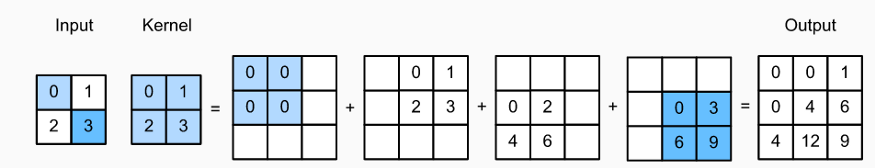
\includegraphics[width=1\textwidth]{resources/cnn/transposed-conv.png}
  \caption{
    Die Komplette Transposed Convolution Operation
    \cite{zhang2020dive}
  }
  \label{image:transposed-conv}
\end{figure}

Jeder Zahl in der Input Matrix wird mit jeder Zahl in den Filter multipliziert. Daraus ergibt sich an jeder Position in der Input Matrix einer 
$ 2 \times 2 $ Matrix. Die überlappende Zahlen auf der Output Matrix werden addiert. Daraus ergibt sich einer $ 3 \times 3 $ Output Matrix.

\subsection{Autoencoder}
Ein Autoencoder ist ein neuronales Netz, welches versucht die Eingangsinformationen zu komprimieren und mit den reduzierten Informationen 
im Ausgang wieder korrekt nachzubilden \cite{was-ist-autoencoder}. Die Komprimierung und Rekonstruktion der Input läuft in zwei Schritten ab, 
weshalb das Netz in zwei Teile betrachtet werden kann.
\\
\subsubsection{Encoder}
Der Encoder reduziert die Dimensionen von einem Input und somit werden die wichtigsten Features in einer reduzierter Dimension komprimiert.
In einem neuronalen Netz wird diese Komprimierung durch die Hidden Layers erreicht. Der Encoder ist definiert als:

\begin{equation}
  h = f(x)
\end{equation}

wobei $x$ einem Input ist, $f$ der Encoder und $h$ die Kodierte Features von $x$.

\subsubsection{Decoder}
Der Decoder ist zuständig für die Rekonstruktion von $x$ anhand $h$ und ist definiert als:

\begin{equation}
  \hat{x} = g(h)
\end{equation}

wobei, $\hat{x}$ der rekonstruierte Input ist, $g$ der Decoder und $h$ die Kodierten Features sind.

In der vorliegende Arbeit werden Autoencoders basierend auf Convolutional Neural Networks eingesetzt.

\section{\textit{Lab}-Farbraum} 
Der \textit{Lab}-Farbraum (auch CIELAB-Farbraum genannt) ist ein Farbraum definiert bei der Internationale
Beleuchtungskommission (\gls{cie}) in 1976. Farben werden mit drei Werte beschrieben. ``\textit{L}'' (Lightness) definiert die Helligkeit.
Die Werte liegen zwischen 0 und 100. ``\textit{a}'' gibt die Farbart und Farbintensität zwischen Grün und Rot und ``\textit{b}'' gibt die
Farbart und Farbintensität zwischen Blau und Gelb. Die Werte für ``\textit{a}'' und ``\textit{b}'' liegen zwischen -128 und 127.
\\
In der vorliegende Arbeit wird den \textit{Lab}-Farbraum verwendet, da es unkompliziert ist, den ``\textit{L}'' Kanal von beide Farbkanäle 
``\textit{a}'' und ``\textit{b}'' zu trennen. Außerdem bildet den \textit{Lab}-Farbraum das Menschliche Sehvermögen besser als den RGB-Farbraum ab.

\section{Verwandte Arbeiten}
Vor der Erstellung dieser Arbeit wurden Methoden von Image Colorization bereits untersucht. Frühere Methoden waren stark an Menschliches Input
gebunden. Der Methode von Levin et al. verwendet Farbstiche auf dem Graustufenbild die Automatisch von einem Algorithmus über das gesamte 
Bild propagiert werden \cite{10.1145/1015706.1015780}.
\\
\\
Der Fokus dieser Arbeit ist auf volle automatische Image Colorization Methoden gesetzt. Konservative Methoden die Convolutional Neural Networks verwenden,
versuchen die Farben von dem Originalen Bild wiederherzustellen in dem die \gls{loss function} die Distanz der vorhergesagte Farbe und die 
Reale Farbe berechnet. Diese Methoden liefern in der Regel entsättigte und blasse Bilder wie bei \cite{zbulak2019image}. Einer der Gründe 
für diese Ergebnissen ist dass die Modelle nicht richtig lernen. Zum Beispiel, Äpfel können verschiedene Farben einnehmen, wie Rot oder Grün. Wenn das 
Netzwerk mit einem MSE Loss trainiert wird, wird der Output bei einem Apfel eine Farbe zwischen Rot und Grün sein, was ein entsättigtes Bild erzeugen wird.
\\
\\
Aus diesem Grund ist das Problem von Image Colorization ein Multimodales Problem, da gleiche Objekte verschiedene Farbe haben können.
Die vorliegende Arbeit orientiert sich auf die Methoden von Zhang et al. und Billaut et al., die ähnliche Ansätze für Image Colorization vorschlagen.
Sie betrachten das Problem als ein Klassifizierungsproblem und trainieren eine CNN mit der Weighted Cross Entropy Loss. Der Output von dem Netzwerk ist 
eine Wahrscheinlichkeitsverteilung über die mögliche Farben für jeden Pixel. Außerdem wird der Loss während des Trainings gewichtet um seltene 
Farben zu bevorzugen.
\\
\\
Beide Ansätze verwenden ``Color \gls{bin}s'' die es unkompliziert ermöglichen das CNN mit der Weighted Cross Entropy Loss zu Trainieren. 
Es wird im nächsten Kapitel weiter auf diese Methode eingegangen.
